\section{Diseño Arquitectónico}
\label{sc:DA}

\subsection{Tecnologías utilizadas}
\label{ssc:tech}

El sistema se compone de tres módulos principales, cada uno encargado de una función especifica dentro del flujo de análisis de ulceras.
\subsection{Backend}
\begin{description}
    \item[Función] Exponer un conjunto de servicios REST para gestionar usuarios, pacientes, imágenes y segmentaciones. 
    \item[Persistencia] Un ORM sobre MySQL facilita la definición de las entidades de dominio y sus relaciones 
    \item[Seguridad] Autentificación mediante tokens, junto con un mecanismo de hashing para las credenciales.
    \item[Manejo de archivos] Recepción, almacenamiento y registro de imágenes y mascaras de segmentación.
    \item[Integración con el modelo de ML] Invoca de forma transparente la lógica de análisis y segmentación desarrollada en Python   
\end{description}

\subsection{Frontend}
\begin{description}
\item[Función] Ofrecer una interfaz web para autenticación, visualización de pacientes y gestión de resultados.
\item[Rendimiento y experiencia] Renderizado inicial en servidor y enrutamiento automático para mejorar tiempos de carga y SEO.
\item[Comunicación] Consumo de los servicios del backend, adjuntando el token de autenticación en cada solicitud.
\item[Componentes] Elementos reutilizables para formularios de acceso, panel de imágenes y tablas de datos.
\end{description}

\subsection{Categorizador}
\begin{description}
\item[Función] Ejecución de algoritmos de visión por computador y machine learning para segmentar imágenes y calcular puntajes clínicos.
\item[Tecnologías] Bibliotecas especializadas en procesamiento de imágenes y aprendizaje automático.
\item[Modo de operación]
\begin{itemize}
\item Segmentación de la zona lesionada.
\item Evaluación y asignación de un puntaje en la escala PWAT.
\end{itemize}
\item[Salida] Máscaras segmentadas y valores de puntuación, disponibles para su consulta en el sistema.
\end{description}

\subsection{Visión Unificada}
Este enfoque modular garantiza:
\begin{itemize}
\item Desarrollo y despliegue independientes por componente.
\item Mantenibilidad y escalabilidad a medida que evolucionan los requerimientos.
\item Aprovechamiento de cada tecnología en su área de fortaleza: servicios web, interfaces dinámicas y modelos de inteligencia artificial.
\end{itemize}



\subsection{Flujo de datos / Vista de alto nivel}
\label{ssc:flow}

Para comprender el funcionamiento global de la plataforma, se describira el recorrido que sigue la información desde el momento en que el usuario inicia una acción hasta que obtiene el resultado final. Esta visión de alto nivel permite apreciar de forma clara y ordenada los componentes implicados y la secuencia de procesos que garantizan el correcto manejo de imágenes, metadatos y resultados de segmentación.

En primer lugar, el usuario interactúa mediante la interfaz web, donde sus solicitudes (por ejemplo, carga de imágenes o consulta de resultados previos) son capturadas y enviadas al servidor. A continuación, el módulo de frontend traduce estas peticiones a llamadas a la API REST, incorporando el token de autenticación para validar el acceso. 

El backend recibe la petición, valida los datos y coordina dos tareas principales:  
\begin{enumerate}
  \item \emph{Persistencia}: guarda o recupera los datos relevantes (tipo de usuario: paciente, imágenes, máscaras) en la base de datos.
  \item \emph{Análisis}: cuando se solicita segmentación o cálculo de puntaje, despacha la petición al módulo de categorización, ejecutando el proceso de visión por computador y machine learning en Python.
\end{enumerate}

El módulo de categorizador procesa la imagen, genera la máscara de la lesión y calcula el puntaje clínico, devolviendo estos resultados al backend. Finalmente, el backend almacena la nueva información y responde al frontend con los datos actualizados, que se presentan al usuario mediante componentes interactivos.  

De este modo, el flujo de datos se organiza en cuatro fases —recolección, procesamiento, persistencia y visualización—, garantizando un tránsito de información seguro, escalable y transparente para el investigador o profesional clínico que utilice la plataforma. La Figura \ref{fig:arquitectura-alto-nivel} ilustra estos pasos en un diagrama de alto nivel.  

\begin{figure}[H]
  \centering
  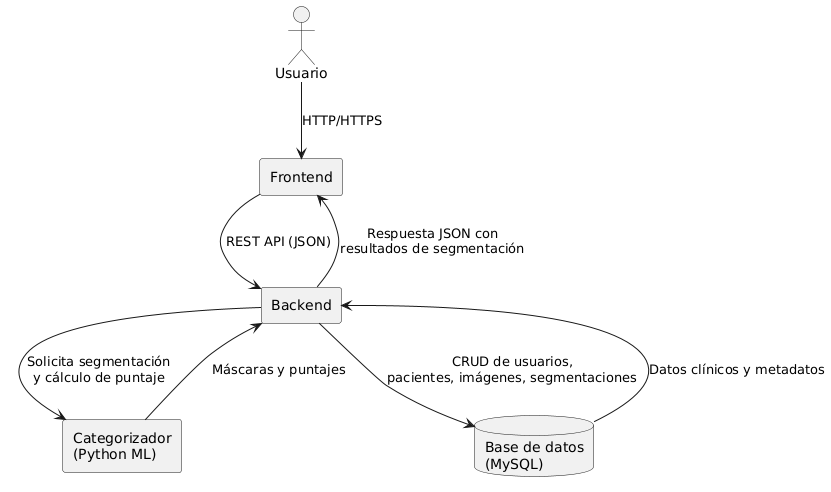
\includegraphics[width=0.8\textwidth,height=0.5\textheight,keepaspectratio]{imagenes/esquemaAlto.png}
  \caption{Esquema de alto nivel del sistema.}
  \label{fig:arquitectura-alto-nivel}
\end{figure}


\subsection{Diagrama de despliegue}
\label{ssc:diagDesp}

\subsubsection{Cliente Web}
Este nodo representa el navegador del usuario, donde se ejecuta la aplicación SPA \footnote{SPA: Single Page Application, es un tipo de aplicación web que se carga una sola vez en el navegador y luego interactúa con el usuario actualizando dinámicamente el contenido de la página sin necesidad de recargarla por completo} construida con Next.js y React. Depende de los artefactos estáticos generados (HTML, CSS y JavaScript) agrupados en un paquete de frontend. La comunicación se realiza sobre HTTP/HTTPS hacia el servidor de la aplicación, enviando solicitudes de carga de imágenes, autentificación y recuperación de datos. Al existir rutas automáticas y rende rizado inicial en servidor, el cliente recibe primero HTML pre-renderizado y luego gestiona de forma reactiva las interacciones con la interfaz

\subsubsection{Servidor de Aplicación}
Agrupa dos paquetes lógicos: el frontend de Next.js y el backend de Express. El paquete de frontend sirve los ficheros estáticos y gestionará el SSR; el de backend expone una API REST para CRUD de usuarios, imágenes y segmentaciones. Internamente, ambos comparten dependencias de Node.js y se despliegan como un mismo contenedor o instancia, garantizando coherencia entre presentación y lógica de negocio. El backend recibe peticiones JSON del cliente, valida tokens y enruta las operaciones según la capa de persistencia o la de análisis.

\subsubsection{Servidor de ML (Categorizador)}
Aislado en una máquina que ejecuta un entorno Python con bibliotecas de visión por computador (OpenCV, PIL, pyradiomics) y aprendizaje automático (scikit-learn, XGBoost, TensorFlow/Keras). Depende de un entorno gestionado por \texttt{Conda} que agrupa todos los módulos necesarios. La interacción con el servidor de aplicación es síncrona: este último envía la imagen a procesar y recibe de vuelta la máscara segmentada y el puntaje PWAT en formato JSON o archivos. De este modo, la lógica de machine learning permanece desacoplada de Node.js.

\subsubsection{Servidor de Base de Datos}
Un servicio MySQL que persiste toda la información clínica y metadatos de imágenes, máscaras y resultados. El backend utiliza un ORM (Sequelize) y el driver mysql2 para comunicarse con este nodo, ejecutando operaciones CRUD. La conexión viaja por la red interna usando el protocolo MySQL; así se separa la capa de datos de las capas de aplicación y análisis, permitiendo escalado independiente y facilidades de respaldo.

\begin{figure}[H]
    \centering
    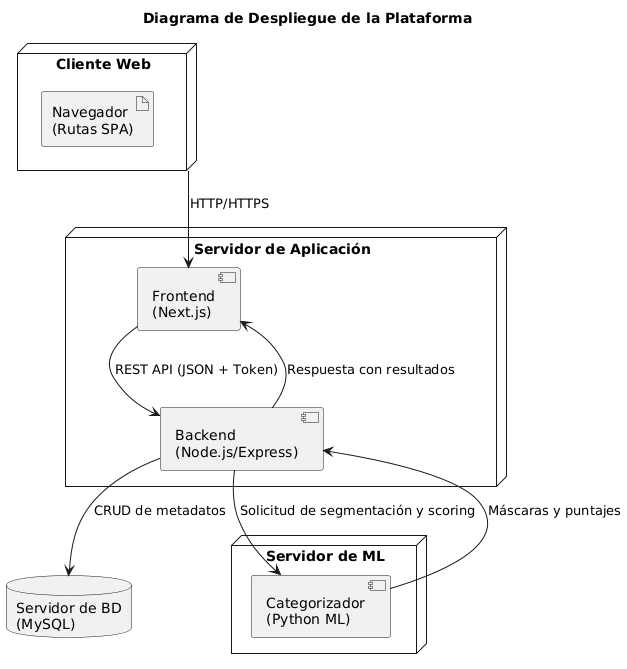
\includegraphics[width=0.8\textwidth,height=0.5\textheight,keepaspectratio]{imagenes/despliegue.png}
    \caption{Diagrama de Despliegue}
    \label{fig:DD}
\end{figure}


\subsection{Diagrama de componentes}
\label{ssc:diaComp}

A continuacion se presenta el diagrama de componentes que sintetiza la organización modular de la plataforma. En el se identifican las unidades lógicas (Frontend, Backend, Categorizador y sistemas de almacenamiento) y los contratos de servicio (interfaces) que establecen sus puntos de interacción. Esta representación y el flujo de dependencias entre los distintos subsistemas.


\begin{figure}[H]
    \centering
    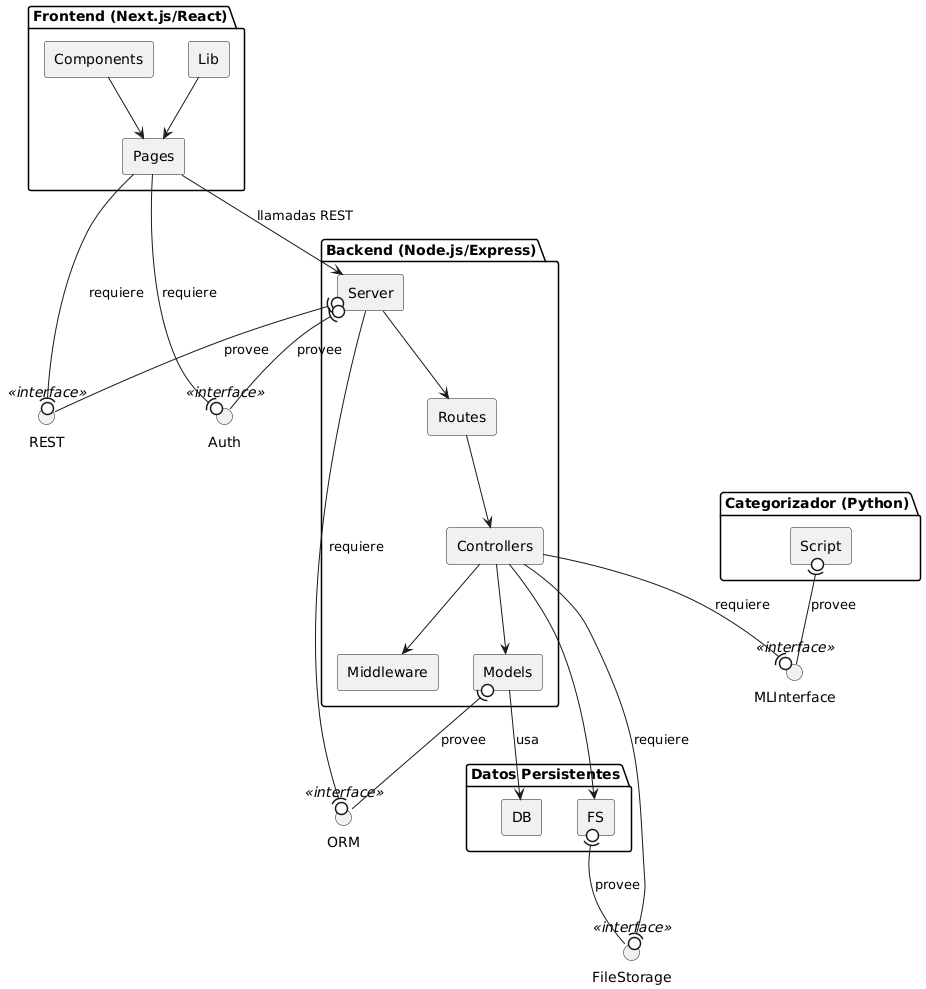
\includegraphics[width=0.7\linewidth]{imagenes/componentes.png}
    \caption{Diagrama de Componentes}
    \label{fig:componentDiagram}
\end{figure}
    
    
    
\subsection{Diagrama de paquetes}
\label{ssc:pack}
    
A continuación se presenta el diagrama de paquetes que ofrece una visión de alto nivel de la estructura modular del sistema. Cada recuadro agrupa elementos relacionados —páginas, componentes, utilidades y estilos del frontend; configuración, middleware, modelos, controladores y rutas del backend; el script de categorización en Python; y los elementos de persistencia de datos— mostrando cómo se organizan y encapsulan las responsabilidades. Las flechas con estereotipos (\texttt{<<uses>>}, \texttt{<<import>>}, \texttt{<<access>>}) indican las dependencias principales entre paquetes: el frontend consume servicios REST del backend, éste orquesta modelos y controladores y lanza el script de PWAT, y finalmente los módulos acceden a la base de datos y al sistema de archivos para leer o almacenar información. Este esquema facilita entender, de un vistazo, qué agrupa cada paquete y cómo fluye la comunicación entre ellos antes de profundizar en los detalles de implementación.

\begin{figure}[H]
    \centering
    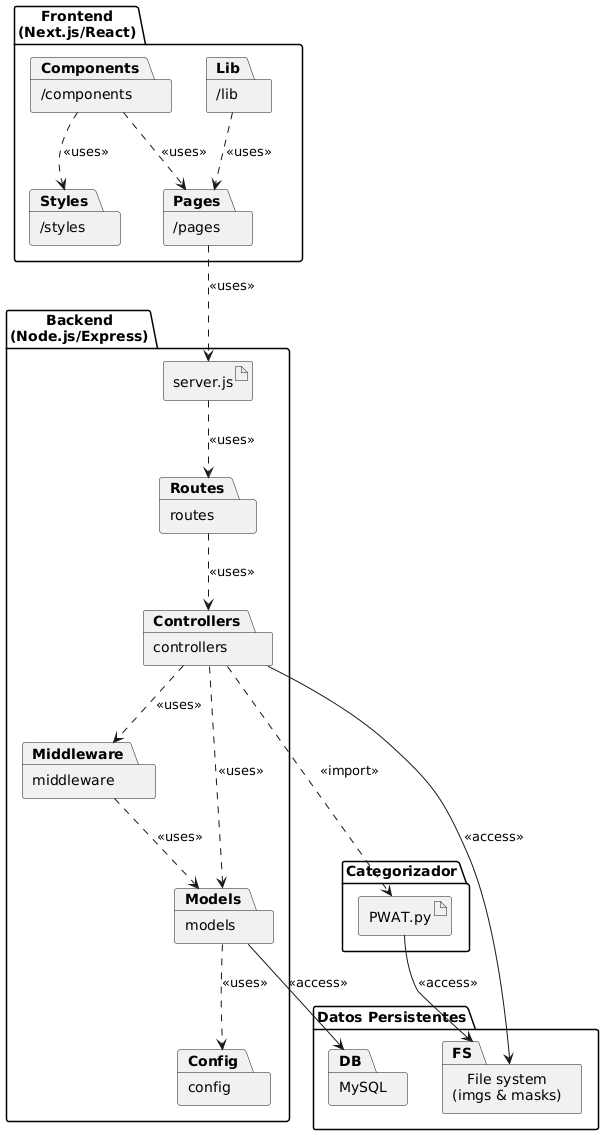
\includegraphics[width=0.7\linewidth]{imagenes/paquetes.png}
    \caption{Diagrama de Paquetes}
    \label{fig:packageDiagram}
\end{figure}
    
\subsection{Diagrama de clases}
\label{ssc:clases}
A continuación se muestra el diagrama de clases que describe el modelo de dominio central de la plataforma. En él aparecen:
Las entidades de gestión de usuarios:
\begin{itemize}
    \item  User
    \item Profesional
    \item Paciente
\end{itemize}
Con sus todos atributos y operaciones principales.

El paquete de contenido clínico
\begin{itemize}
    \item Imagen
    \item Segmentacion
    \item PWATScore
\end{itemize}

Estos modelan la captura, tratamiento y evaluacion de las heridas

Las relaciones y cardinalidades revelan cómo un usuario se vincula a un profesional o paciente, cómo un paciente puede tener múltiples imágenes, y cómo cada imagen da lugar a múltiples segmentaciones y puntuaciones.
Este esquema estático ofrece una visión clara de las piezas independientes del sistema y sus conexiones, sirviendo como referencia para el desarrollo, la integración y la evolución de la plataforma.
\begin{figure}[H]
  \centering
  \adjustbox{%
    max width=\textwidth,       % como mucho el ancho del texto
    max height=1.3\textheight,   % o el 90% de la altura del área imprimible
    keepaspectratio             % sin deformar
  }{%
    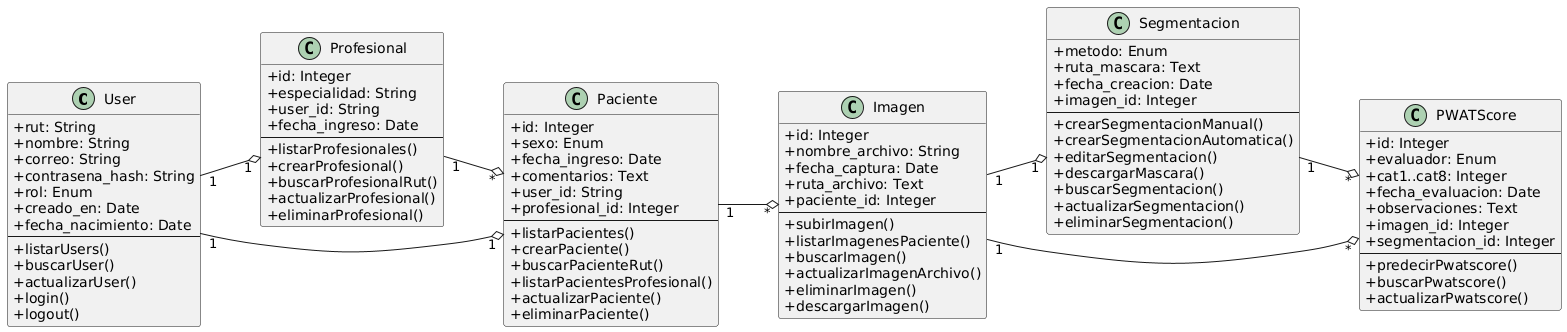
\includegraphics{imagenes/clases.png}%
  }
  \caption{Modelo Relacional}
  \label{fig:classesDiagram}
\end{figure}


\section{Diseño de Datos}
\label{sc:DD}

\subsection{Diagrama Entidad Relación}
\label{ssc:ER}
A continuación se presenta el diagrama entidad-relación en notación de Chen \cite{chen1976entity} que sintetiza la estructura lógica de la base de datos. En él se identifican las seis entidades principales (User, Profesional, Paciente, Imagen, Segmentación y PWATScore), sus atributos clave y las relaciones que las vinculan (EsPaciente, EsProfesional, Atiende, Posee, Genera, Evalua y Deriva), con sus cardinalidades asociadas. Este modelo de alto nivel facilita la comprensión del esquema de almacenamiento de datos antes de pasar a detalles de implementación.
\begin{figure}[H]
    \centering
    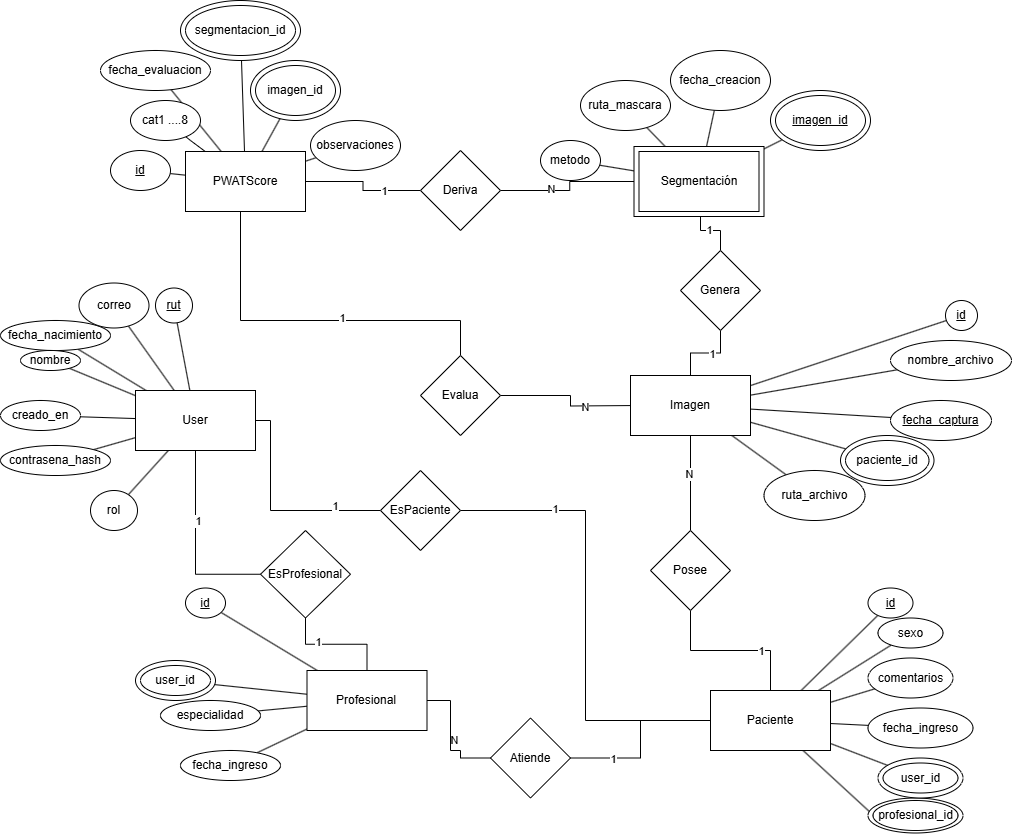
\includegraphics[width=1\linewidth]{imagenes/ER (1).png}
    \caption{Diagrama Entidad Relacion}
    \label{fig:classesDiagram}
\end{figure}

\subsection{Modelo Relacional}
\label{ssc:Rel}

A continuación se presenta el modelo relacional que refleja la implementación en MySQL de las entidades y relaciones definidas en el esquema ER. Cada rectángulo representa una tabla con sus columnas y restricciones principales (PK, FK, UQ), mientras que las líneas indican las relaciones entre tablas con sus cardinalidades (1:1, 1:N). Este diagrama facilita la lectura de la estructura de la base de datos y sirve de guía para generar las sentencias DDL\footnote{DDL: Data Definition Language o Lenguaje de Definicion de Datos.} correspondientes.
\begin{figure}[H]
  \centering
  \adjustbox{%
    max width=\textwidth,       % como mucho el ancho del texto
    max height=0.70\textheight,   % o el 90% de la altura del área imprimible
    keepaspectratio             % sin deformar
  }{%
    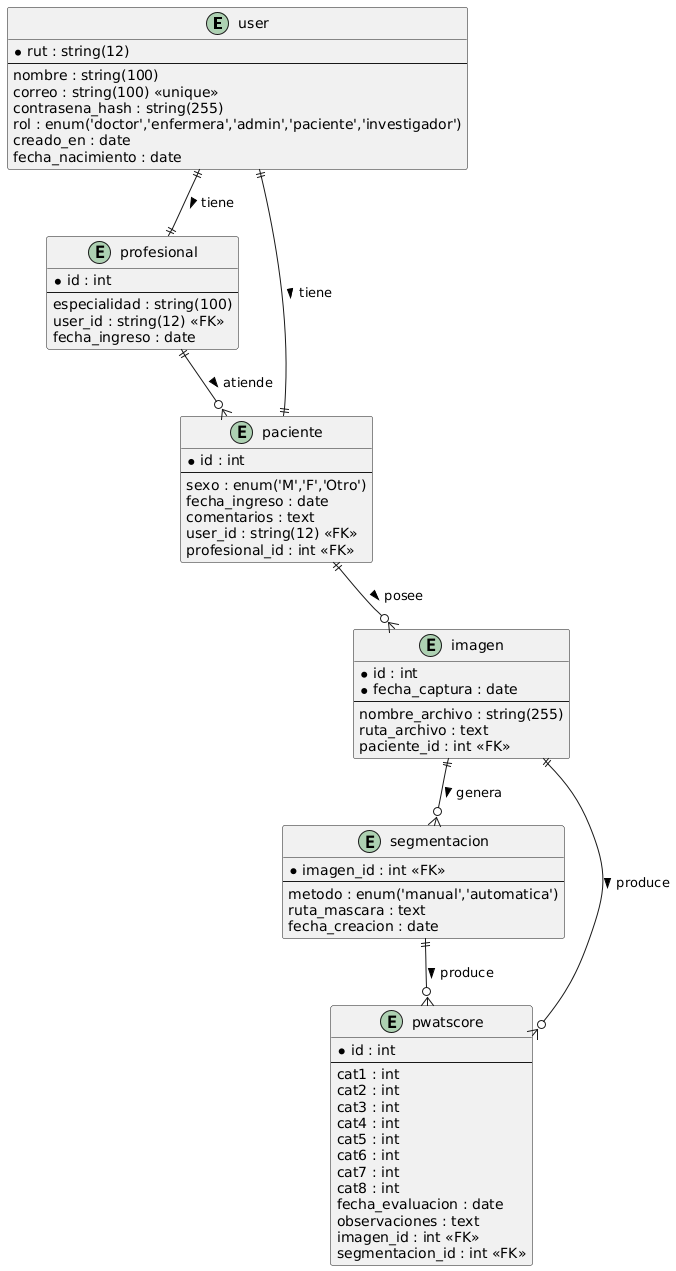
\includegraphics{imagenes/relacional.png}%
  }
  \caption{Modelo Relacional}
  \label{fig:classesDiagram}
\end{figure}



\subsection{Diccionario de Datos}
\label{ssc:DD}
A continuación se incluye el Diccionario de Datos de la base de datos relacional. En él se describen de forma detallada cada una de las tablas —con sus claves primarias, foráneas y restricciones de unicidad— así como los atributos que las componen, su tipo de datos y su significado dentro del sistema. Este artefacto sirve como referencia para el equipo de desarrollo y como documentación formal de la estructura de almacenamiento, facilitando la generación de los scripts DDL y garantizando la consistencia e integridad de la información durante todo el ciclo de vida del proyecto.

\renewcommand{\arraystretch}{1.0}   % Menos altura de fila

\subsection*{Tabla \texttt{User}}
{\footnotesize
\begin{tabularx}{\textwidth}{l l l X}
\hline
\textbf{Atributo} & \textbf{Tipo} & \textbf{Restricción} & \textbf{Descripción} \\\hline
rut               & VARCHAR(20)   & PK                   & RUT del usuario, único e identifica al usuario. \\
nombre            & VARCHAR(100)  & —                    & Nombre completo. \\
correo            & VARCHAR(150)  & UQ                   & Correo electrónico. \\
contrasena\_hash  & VARCHAR(255)  & —                    & Hash de la contraseña. \\
rol               & ENUM          & —                    & Perfil (\texttt{admin}, \texttt{profesional}, \texttt{paciente}). \\
creado\_en        & DATETIME      & —                    & Fecha de creación. \\
fecha\_nacimiento & DATE          & —                    & Fecha de nacimiento. \\\hline
\end{tabularx}
}

\subsection*{Tabla \texttt{Profesional}}
{\footnotesize
\begin{tabularx}{\textwidth}{l l l X}
\hline
\textbf{Atributo} & \textbf{Tipo}       & \textbf{Restricción} & \textbf{Descripción} \\\hline
id                & INT AUTO\_INCREMENT & PK                   & Identificador único. \\
user\_id          & VARCHAR(20)         & FK                   & RUT del usuario. \\
especialidad      & VARCHAR(100)        & —                    & Área de especialidad. \\
fecha\_ingreso    & DATE                & —                    & Fecha de alta. \\\hline
\end{tabularx}
}

\subsection*{Tabla \texttt{Paciente}}
{\footnotesize
\begin{tabularx}{\textwidth}{l l l X}
\hline
\textbf{Atributo} & \textbf{Tipo}              & \textbf{Restricción}  & \textbf{Descripción} \\\hline
id               & INT AUTO\_INCREMENT        & PK                    & Identificador del paciente. \\
sexo             & ENUM                       & —                     & Sexo biológico (\texttt{M}, \texttt{F}). \\
fecha\_ingreso   & DATE                       & —                     & Fecha de registro. \\
comentarios      & TEXT                       & —                     & Notas o comentarios. \\
user\_id         & VARCHAR(20)                & FK                    & RUT de usuario. \\
profesional\_id  & INT                        & FK                    & Profesional a cargo. \\\hline
\end{tabularx}
}

\subsection*{Tabla \texttt{Imagen}}
{\footnotesize
\begin{tabularx}{\textwidth}{l l l X}
\hline
\textbf{Atributo} & \textbf{Tipo}            & \textbf{Restricción} & \textbf{Descripción} \\\hline
id               & INT AUTO\_INCREMENT      & PK                   & Identificador de imagen. \\
fecha\_captura   & DATETIME                 & PK                   & Marca temporal. \\
nombre\_archivo  & VARCHAR(200)             & —                    & Nombre de fichero. \\
ruta\_archivo    & TEXT                     & —                    & Ruta en disco. \\
paciente\_id     & INT                      & FK                   & Paciente asociado. \\\hline
\end{tabularx}
}

\subsection*{Tabla \texttt{Segmentacion}}
{\footnotesize
\begin{tabularx}{\textwidth}{l l l X}
\hline
\textbf{Atributo} & \textbf{Tipo}            & \textbf{Restricción} & \textbf{Descripción} \\\hline
metodo           & ENUM                      & —                    & Tipo (\texttt{manual}, \texttt{automatica}). \\
ruta\_mascara    & TEXT                     & —                    & Ruta de la máscara. \\
fecha\_creacion  & DATETIME                 & —                    & Fecha de creación. \\
imagen\_id       & INT                      & FK PK                  & Imagen asociada. \\\hline
\end{tabularx}
}

\subsection*{Tabla \texttt{PWATScore}}
{\footnotesize
\begin{tabularx}{\textwidth}{l l l X}
\hline
\textbf{Atributo}      & \textbf{Tipo}         & \textbf{Restricción} & \textbf{Descripción} \\\hline
id                    & INT AUTO\_INCREMENT   & PK                   & ID del registro. \\
cat1–cat8             & INT                   & —                    & Categorías clínicas (1–8). \\
fecha\_evaluacion     & DATETIME              & —                    & Fecha de evaluación. \\
observaciones         & TEXT                  & —                    & Comentarios adicionales. \\
imagen\_id            & INT                   & FK                   & Imagen evaluada. \\
segmentacion\_id      & INT                   & FK                   & Segmentación usada. \\\hline
\end{tabularx}
}

\subsection{Diagrama de Flujo de datos}

A continuación se describe el recorrido de la información a través de los distintos módulos de la plataforma:

\begin{enumerate}
  \item \textbf{Interacción de usuario y Frontend}  
    Los componentes de la interfaz (botones, formularios, listados) y las páginas de Next.js reciben las acciones del usuario (por ejemplo, carga de imagen o petición de historial). Estas páginas utilizan el helper de API (\texttt{api.js}) para generar peticiones REST al servidor, adjuntando el token JWT para autorizar cada solicitud.
  
  \item \textbf{Procesamiento en el Backend}  
    El servidor Express recibe cada solicitud y la enruta según su endpoint. A través de las capas de rutas y controladores se valida la entrada, se gestionan credenciales y se aplican reglas de negocio. Los controladores interactúan con los modelos Sequelize para leer o escribir datos en la base de datos MySQL.
  
  \item \textbf{Gestión de archivos y análisis}  
    Cuando corresponde, los controladores también almacenan o recuperan imágenes y máscaras en el sistema de archivos. Para la segmentación automática y el cálculo del PWATScore, el backend invoca de forma asíncrona el script de Python (\texttt{PWAT.py}), pasando la ruta del archivo. El script procesa la imagen, genera las máscaras y devuelve los resultados, que se guardan nuevamente en disco.
  
  \item \textbf{Respuesta al Frontend}  
    Una vez completado el procesamiento —persistencia en la base de datos, almacenamiento de archivos y análisis de ML— el backend construye la respuesta JSON con los datos solicitados (por ejemplo, URLs de las máscaras, valores de puntaje). El frontend recibe estos datos y los muestra en la interfaz, ofreciendo al usuario un feedback inmediato y la posibilidad de seguir navegando o realizar nuevas acciones.
\end{enumerate}

\begin{figure}[H]
    \centering
    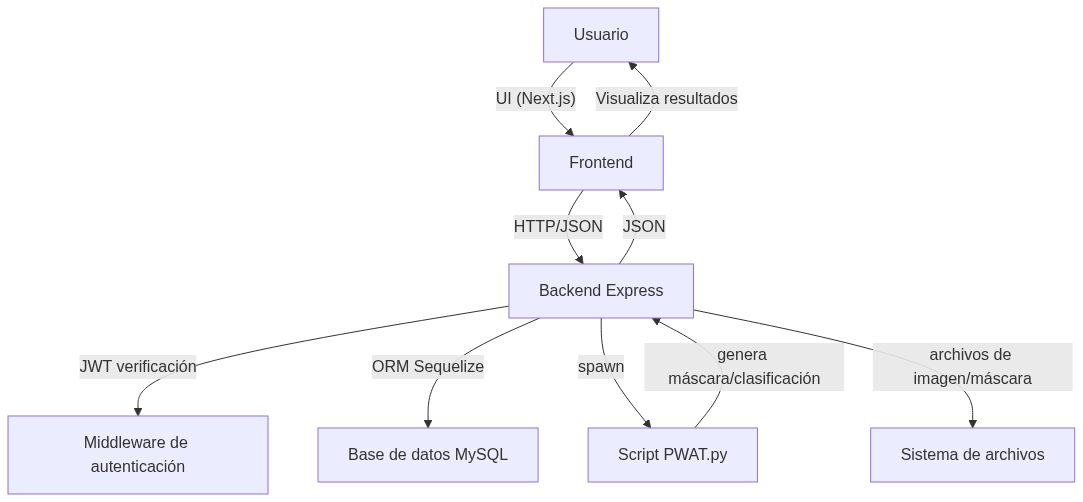
\includegraphics[width=1\linewidth]{imagenes/flujo.png}
    \caption{Modelo Relacional}
    \label{fig:classesDiagram}
\end{figure}

\section{Diseño de Interfaz}
\label{sc:DI}

Para prensetar el alcance de la aplicaciom de gestion y revision de imagenes, se empleo un esquema de interfaces de alto nivel, mostrando a su alrededor los cuatro actores principales: \textbf{Administrador}, \textbf{Profesional}, \textbf{Investigador} y \textbf{Paciente}. Cada uno de ellos interactua con el interfaz web (implementada en React/Next.js) para realizar su funcionalidad especifica: el \textbf{Administrador} gestiona usuarios y asignaciones, el \textbf{Investigador} consulta metricas y lanza procesos de rentremamiento, el \textbf{Profesional} lista pacientes y sube o reemplaza imagenes, y el \textbf{Paciente} edita su perfil y revisa sus historiales.


\begin{figure}[H]
    \centering
    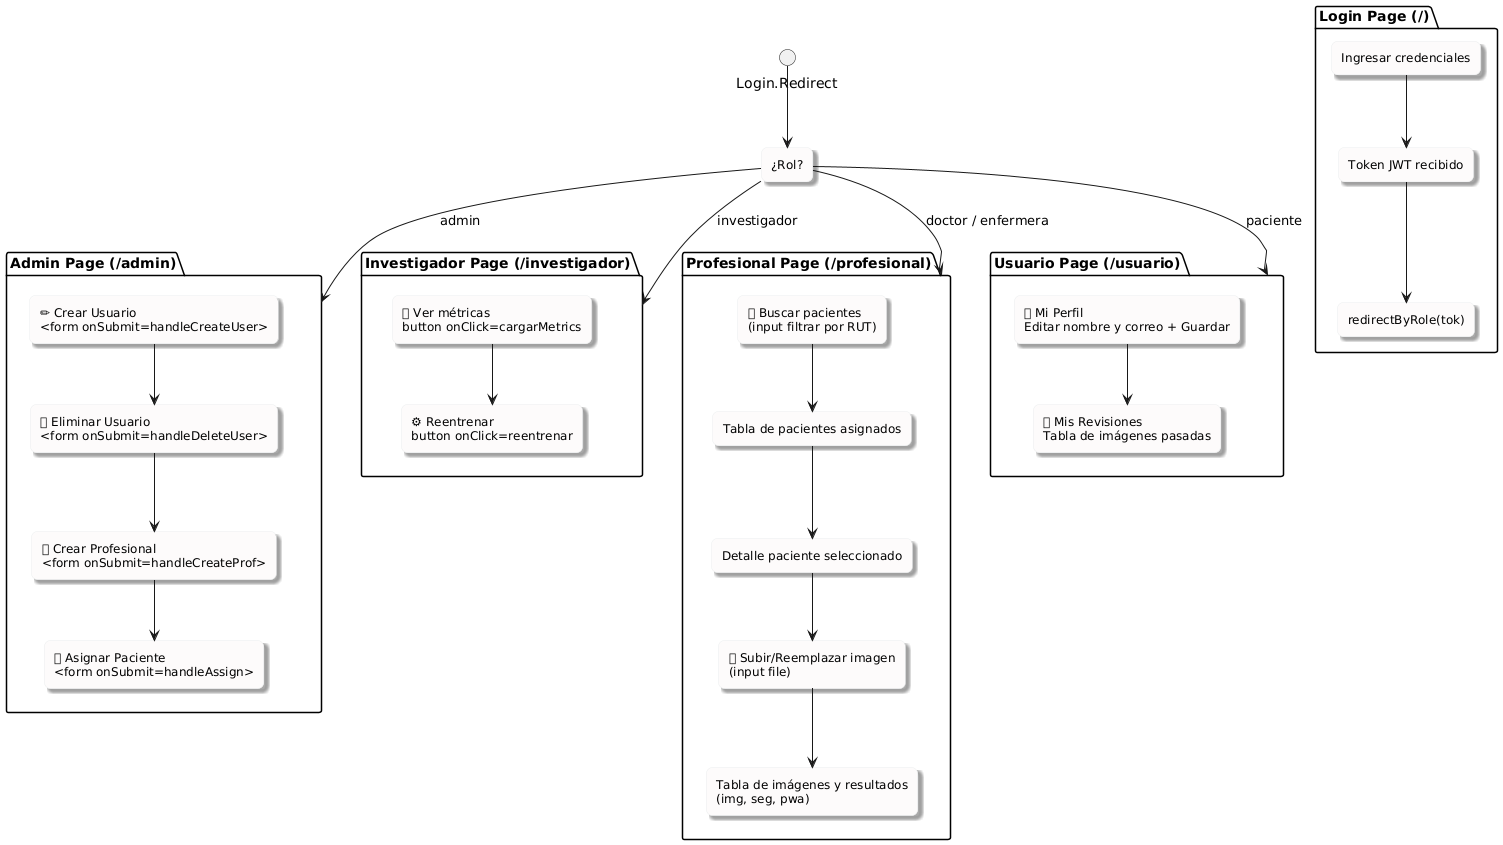
\includegraphics[width=1\linewidth]{imagenes/esquema.png}
    \caption{Modelo Relacional}
    \label{fig:classesDiagram}
\end{figure}


%\subsection{Prototipos de Interfaces Gráficas}
%\label{ssc:IGraph}


\section{Diseño de Pruebas}
\label{sc:DP}

Este plan de pruebas se estructura según los principales módulos del sistema: Backend (Node.js/Express), Frontend (Next.js) y Categorizador (Python). Cada componente tiene pruebas asociadas para asegurar su correcto funcionamiento, integración y robustez frente a errores

\subsubsection{Backend}
\textbf{Cobertura de pruebas}
\begin{itemize}
    \item Pruebas Unitarias:
    \begin{itemize}
        \item Cada controlador cuenta con pruebas especificas que verifiquen el comportamiento aislado de sus funciones principales
    \end{itemize}
\begin{itemize}
    \item Se utilizan herramientas como Supertest para simular el entorno de ejecución y mockear dependencias externas
    \item Conexión y operaciones en base de datos de pruebas o uso de mocks de Sequelize
    \item Validación de relaciones entre modelos y respuestas ante inconsistencias
\end{itemize}
\end{itemize}

\subsubsection{Frontend}
\textbf{Cobertura de pruebas}
\begin{itemize}
    \item Pruebas de componentes
    \begin{itemize}
        \item Validación de renderizado correcto y comportamiento de componentes
    \end{itemize}
\begin{itemize}
    \item Simulación de interacciones en formularios
\end{itemize}
\begin{itemize}
    \item Validación de que las peticiones incluyen correctamente los tokens de autenticación
    \item Flujo completo desde login hasta la evaluación de la ulcera
\end{itemize}
\end{itemize}
\subsubsection{Categorizador}
\textbf{Cobertura de pruebas}
\begin{itemize}
    \item Pruebas unitarias
    \begin{itemize}
        \item Escritura y lectura de archivos de imagen y mascaras
        \item Funciones como \texttt{predecir\_mascara}, \texttt{predecir} y \texttt{mask\_predict} se prueban de forma aislada
    \end{itemize}
\end{itemize}

\subsection{Pruebas Unitarias}
\label{ssc:UT}

\begin{enumerate}
    \item \textbf{Backend}
    \begin{enumerate}
        \item \texttt{User.crearUser} debe crear un nuevo usuario con datos validos
        \item \texttt{User.listarUsers} debe retornar todos los usuarios desde la base de datos
        \item \texttt{Pacientes.crearPaciente} debe validar datos requeridos y retornar error si falta
        \item \texttt{Segmentacion.crearSegmentacion} debe recibir la imagen y generar peticion al categorizador
        \item \texttt{PWATScore.calcularPWAT} debe devolver correctamente el puntaje basado en la mascara
    \end{enumerate}
\item \textbf{Frontend}
\begin{enumerate}
    \item Componentes Visuales
    \begin{enumerate}
        \item \texttt{LogiutButton} ejecuta correctamente la función de cierre de sesión
    \end{enumerate}
\item Paginas y Formularios
\begin{enumerate}
    \item \texttt{pages/index.js} redirige al dashborad correcto según rol retornado por la API
    \item Formularios manejan inputs vacíos o inválidos con mensajes adecuados
\end{enumerate}
\item Logica de API
\begin{enumerate}
    \item \texttt{lib/api.js} incluyen correctamente el token en cabeceras
    \item Maneja errores HTTP con feedback al usuario
\end{enumerate}
\end{enumerate}
\item \textbf{Categorizados}
\begin{enumerate}
    \item Funcion de prediccion
    \begin{enumerate}
        \item \texttt{predecir\_mascara} retorna una máscara  valida dado un input conocido
        \item \texttt{predecir} returna una clasificación esperada para inputs de prueba
    \end{enumerate}
\item Errores y Casos Borde
\begin{enumerate}
    \item Responde adecuadamente ante archivos faltantes, rutas invalidas o formatos erróneos
\end{enumerate}
\end{enumerate}
\end{enumerate}

\subsection{Pruebas de Integración}
\label{ssc:IT}

\begin{itemize}
    \item \textbf{Backend}
    \begin{itemize}
        \item Se verifica el funcionamiento conjunto de rutas, middlewares y controladores:
        \begin{itemize}
            \item Pruebas en endpoints como \texttt{POST /users/login}, \texttt{POST /pacientes}, \texttt{POST /segmentaciones}
            \item Confirmación de direccional de errores desde middleware a manejo centralizado
            \item Verificación de acceso a base de datos y correcta respuesta HTTP
        \end{itemize}
    \end{itemize}
\item \textbf{Frontend}
\begin{itemize}
    \item Pruebas sobre la interacción entre componentes, navegación y llamadas a la API
    \begin{itemize}
        \item Confirmación de navegación al dashboard tras autenticación correcta
        \item Validación del comportamiento al recibir errores del backend
        \item Coordinación entre hooks, rutas, y APIs simuladas para pruebas
    \end{itemize}
\end{itemize}
\item \textbf{Categorizador}
\begin{itemize}
    \item Ejecución integrada desde backend Node.js
    \begin{itemize}
        \item Invocación mediante \texttt{child\_process.spawn} o \texttt{conda run}
        \item Recepción y parseo correcto de la respuesta del script \texttt{Python}
        \item Validación de datos temporales generados (mascaras, predicciones)
    \end{itemize}
\end{itemize}
\end{itemize}



\subsection{Pruebas con Usuarios}
\label{ssc:PU}


Este plan evalúa la experiencia de uso del sistema desde la perspectiva de distintos perfiles de usuario: administradores, profesionales de salud y pacientes. Se realizarán pruebas de usabilidad, cumplimiento de flujos esperados y validación de restricciones de acceso.

\subsubsection{Escenarios por Rol}

\begin{itemize}
    \item \textbf{Administrador:}
    \begin{itemize}
        \item Acceso al panel de gestión de usuarios y profesionales.
        \item Creación, edición y eliminación de cuentas.
        \item Acceso completo al historial de segmentaciones.
    \end{itemize}
    
    \item \textbf{Profesional de Salud:}
    \begin{itemize}
        \item Ingreso con credenciales válidas.
        \item Registro de nuevos pacientes.
        \item Carga de imágenes para segmentación.
        \item Visualización de resultados de PWAT.
    \end{itemize}
    
    \item \textbf{Paciente:}
    \begin{itemize}
        \item Acceso restringido a sus propias evaluaciones.
        \item Visualización de resultados previos.
    \end{itemize}
\end{itemize}

\subsubsection{Criterios de Aceptación}

\begin{itemize}
    \item Navegación fluida y sin errores.
    \item Mensajes de retroalimentación claros ante errores o validaciones.
    \item Respeto de los permisos asignados a cada tipo de usuario.
    \item Correcta visualización de resultados y datos asociados.
\end{itemize}

\subsection{Instrumentos}

\begin{itemize}
    \item Pruebas manuales con checklist por escenario.
    \item Grabación de sesiones de prueba para análisis posterior.
    \item Encuesta de satisfacción y usabilidad (\textbf{NASA-TLK} \cite{Hart1988}) aplicada a usuarios reales.
\end{itemize}

\subsection{Definición de métricas de apoyo}\label{ssc:DMA}

Las siguientes métricas permiten cuantificar el desempeño del sistema, evaluar la calidad del software y apoyar la toma de decisiones durante la validación con la escala \textbf{NASA-TLK}:

\begin{itemize}
\item \textbf{Cobertura de pruebas}  \
p. ej. 85\%  \
Porcentaje de funciones, flujos y rutas críticas cubiertas por pruebas automáticas (unitarias, de integración y funcionales).
\item \textbf{Tasa de éxito en pruebas unitarias e integración}  \\
p. ej. 98\%  \\
Número de pruebas que pasan sobre el total de pruebas ejecutadas en cada ciclo.

\item \textbf{Tiempo promedio de respuesta}  \\
p. ej. Login: 250\,ms; Segmentación: 500\,ms; Evaluación: 750\,ms  \\
Promedio de latencia medido en endpoints clave en escenarios de carga realista.

\item \textbf{Tasa de errores encontrados por usuarios}  \\
p. ej. 2 incidencias por ciclo de pruebas  \\
Número de defectos o fallos reportados durante las sesiones de pruebas con usuarios (ambiente de validación).

\item \textbf{Puntuación NASA-TLK}  \\
p. Escala de 1 a 7 por dimensión  \\
Evaluación estandarizada de usabilidad centrada en:  \\
   \begin{itemize}
       \item \textbf{Carga Mental}
       \item \textbf{Carga Física}
       \item \textbf{Carga Temporal}
       \item \textbf{Desempeño}
       \item \textbf{Esfuerzo}
       \item \textbf{Satisfacción}
       \item \textbf{Curva de Aprendizaje}
   \end{itemize}
Se recogen las valoraciones de los usuarios tras completar tareas esenciales.
\end{itemize}

\noindent\textbf{Uso y frecuencia de análisis:}
\begin{itemize}
\item Se calculan tras cada iteración de pruebas de usabilidad para identificar áreas críticas de mejora.
\item Se comparan tendencias temporales para validar estabilidad y evolución de la experiencia clínica.

\end{itemize}
